\subsection{Selección de diseño conceptual}

Con base en la tabla AHP, después de haber realizado las ponderaciones de acuerdo a los criterios anteriormente mencionados, se obtuvieron los componentes que mejor se adaptaban y que cumplen con las necesidades del proyecto; estos componentes se presentan en la tabla \ref{tab:modeloselec}.

De igual forma, se realizó una discusión para realizar el boceto que englobe mejor las soluciones. El boceto permite ilustrar el diseño conceptual, modelo a partir del cual se realizaron los diseños de los módulos del sistema. El boceto propuesto está en la ilustración \ref{fg:boceto seleccionado}

\begin{table}[h]
    \centering
    \caption{Modelo seleccionado}
    \begin{tabular}{|c|c|}
         \hline
         \rowcolor[rgb]{ .251,  .251,  .251}{\textcolor[rgb]{ 1,  1,  1}{Características}} & {\textcolor[rgb]{ 1,  1,  1}{Selección}} \\
         \hline
         \rowcolor[rgb]{ .886,  .937,  .855}Trituración & Rallador\\
         \hline
         \rowcolor[rgb]{ .867,  .922,  .969}Almacenamiento & Contenedor horizontal\\
         \hline
         \rowcolor[rgb]{ 1,  .949,  .8}Palas de agitación & Palas planas\\
         \hline
         \rowcolor[rgb]{ .929,  .929,  .929}Trasmisión de movimiento & Banda V\\
         \hline
         \rowcolor[rgb]{ .988,  .894,  .839}Medir temperatura & Sensor electrónico\\
         \hline
         \rowcolor[rgb]{ .886,  .937,  .855}Medir humedad & Sensor ambiental\\
         \hline
         \rowcolor[rgb]{ 1,  .949,  .8}Elevar temperatura & Resistencia eléctrica\\
         \hline
         \rowcolor[rgb]{ .929,  .929,  .929}Elevar humedad & Por goteo\\
         \hline
         \rowcolor[rgb]{ .988,  .894,  .839}Oxigenar el sistema & Ventilación directa\\
         \hline
          \rowcolor[rgb]{ .886,  .937,  .855}Unidad de procesamiento & Tarjeta de desarrollo\\
         \hline
         \rowcolor[rgb]{ .867,  .922,  .969}Interfaz hombre-máquina & Botones y pantalla\\
         \hline
    \end{tabular}
    \label{tab:modeloselec}
\end{table}

%La utilidad de este método es la fácil asignación  de valores de todos los diferentes componentes, ya que al tener una gran cantidad de combinaciones posibles era difícil determinar las mejores opciones al tratarse de un sistema que integra a todos ellos en su funcionamiento.


\begin{figure}[h!]
    \centering
        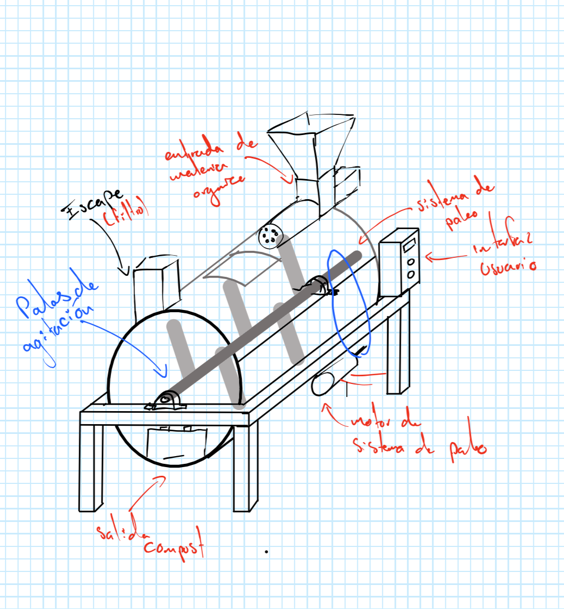
\includegraphics[scale=0.4]{images/Capitulo 3/3.2.5 Diseño Conceptual/Boceto seleccionado.png}
        \caption{Boceto seleccionado}
    \label{fg:boceto seleccionado}
\end{figure}
